% Plantilla para un Trabajo Fin de Grado de la Universidad de Granada,
% adaptada para el Doble Grado en Ingeniería Informática y Matemáticas.
%
%  Autor: Mario Román.
%  Licencia: GNU GPLv2.
%
% Esta plantilla es una adaptación al castellano de la plantilla
% classicthesis de André Miede, que puede obtenerse en:
%  https://ctan.org/tex-archive/macros/latex/contrib/classicthesis?lang=en
% La plantilla original se licencia en GNU GPLv2.
%
% Esta plantilla usa símbolos de la Universidad de Granada sujetos a la normativa
% de identidad visual corporativa, que puede encontrarse en:
% http://secretariageneral.ugr.es/pages/ivc/normativa
%
% La compilación se realiza con las siguientes instrucciones:
%   pdflatex --shell-escape main.tex
%   bibtex main
%   pdflatex --shell-escape main.tex
%   pdflatex --shell-escape main.tex

% Opciones del tipo de documento
\documentclass[oneside,openright,titlepage,numbers=noenddot,openany,headinclude,footinclude=true,
cleardoublepage=empty,abstractoff,BCOR=5mm,paper=a4,fontsize=12pt,main=spanish]{scrreprt}

% Paquetes de latex que se cargan al inicio. Cubren la entrada de
% texto, gráficos, código fuente y símbolofs.
\usepackage[utf8]{inputenc}
\usepackage[T1]{fontenc}
\usepackage{fixltx2e}
\usepackage{graphicx} % Inclusión de imágenes.
\usepackage{grffile}  % Distintos formatos para imágenes.
\usepackage{longtable} % Tablas multipágina.
\usepackage{wrapfig} % Coloca texto alrededor de una figura.
\usepackage{rotating}
\usepackage[normalem]{ulem}
\usepackage{amsmath}
\usepackage{dsfont}
\usepackage{textcomp}
\usepackage{amssymb}
\usepackage{capt-of}
\usepackage[colorlinks=true]{hyperref}
\usepackage{tikz} % Diagramas conmutativos.
\usepackage{minted} % Código fuente.
\usepackage[T1]{fontenc}
\usepackage[numbers]{natbib}

% Plantilla classicthesis
\usepackage[beramono,eulerchapternumbers,linedheaders,parts,a5paper,dottedtoc,
manychapters,pdfspacing]{classicthesis}

% Geometría y espaciado de párrafos.
\setcounter{secnumdepth}{0}
\usepackage{enumitem}
\setitemize{noitemsep,topsep=0pt,parsep=0pt,partopsep=0pt}
\setlist[enumerate]{topsep=0pt,itemsep=-1ex,partopsep=1ex,parsep=1ex}
\usepackage[top=1in, bottom=1.5in, left=1in, right=1in]{geometry}
\setlength\itemsep{0em}
\setlength{\parindent}{0pt}
\usepackage{parskip}

% Profundidad de la tabla de contenidos.
\setcounter{secnumdepth}{3}

% Usa el paquete minted para mostrar trozos de código.
% Pueden seleccionarse el lenguaje apropiado y el estilo del código.
\usepackage{minted}
\usemintedstyle{colorful}
\setminted{fontsize=\small}
\setminted[haskell]{linenos=false,fontsize=\small}
\renewcommand{\theFancyVerbLine}{\sffamily\textcolor[rgb]{0.5,0.5,1.0}{\oldstylenums{\arabic{FancyVerbLine}}}}

% Path para las imágenes
\graphicspath{{figures/}}

% Archivos de configuración.
%------------------------
% Bibliotecas para matemáticas de latex
%------------------------
\usepackage{amsthm}
\usepackage{amsmath}
\usepackage{tikz}
\usepackage{tikz-cd}
\usetikzlibrary{shapes,fit}
\usepackage{bussproofs}
\EnableBpAbbreviations{}
\usepackage{mathtools}
\usepackage{scalerel}
\usepackage{stmaryrd}

%------------------------
% Estilos para los teoremas
%------------------------
\theoremstyle{plain}
\newtheorem{theorem}{Teorema}
\newtheorem{proposition}{Proposición}
\newtheorem{lemma}{Lema}
\newtheorem{corollary}{Corolario}

\theoremstyle{definition}
\newtheorem{definition}{Definición}
\newtheorem{postulate}{Postulado}
\newtheorem*{postulate 3'}{Postulate 3'}
\newtheorem*{postulate 2'}{Projective Measurement}


% Comento estas lineas originales intentando que diga dem
%\renewenvironment{proof}{{\bfseries Proof.}}{\qed}

% Change the proof style so it's in English and add \qed at the end.
%\renewenvironment{proof}{{\bfseries Proof.}}{\qed}

% Añadido por mi intentando que pone "Demostración" y no "Proof"
\renewenvironment{proof}{{\bfseries Demostración.}}{\qed}
\renewenvironment{proof}{{\bfseries Demostración.}}{\qed}
% hasta aqui

\theoremstyle{remark}
\newtheorem{remark}{Remark}
\newtheorem{exampleth}{Ejemplo}

\begingroup\makeatletter\@for\theoremstyle:=definition,remark,plain\do{\expandafter\g@addto@macro\csname th@\theoremstyle\endcsname{\addtolength\thm@preskip\parskip}}\endgroup

%------------------------
% Macros
% ------------------------

\newcommand*{\C}{\mathds{C}}
\newcommand*{\ra}{\rangle}
\newcommand*{\la}{\langle}

% Para poner sonrisa sobre puntos suspensivos. Uso: \overplace{n}{\dotsc}
\newcommand{\overplace}[2]{%
	\overset{\substack{#1\\\smile}}{#2}%
}  % En macros.tex se almacenan las opciones y comandos para escribir matemáticas.
% ****************************************************************************************************
% classicthesis-config.tex 
% formerly known as loadpackages.sty, classicthesis-ldpkg.sty, and classicthesis-preamble.sty 
% Use it at the beginning of your ClassicThesis.tex, or as a LaTeX Preamble 
% in your ClassicThesis.{tex,lyx} with % ****************************************************************************************************
% classicthesis-config.tex 
% formerly known as loadpackages.sty, classicthesis-ldpkg.sty, and classicthesis-preamble.sty 
% Use it at the beginning of your ClassicThesis.tex, or as a LaTeX Preamble 
% in your ClassicThesis.{tex,lyx} with % ****************************************************************************************************
% classicthesis-config.tex 
% formerly known as loadpackages.sty, classicthesis-ldpkg.sty, and classicthesis-preamble.sty 
% Use it at the beginning of your ClassicThesis.tex, or as a LaTeX Preamble 
% in your ClassicThesis.{tex,lyx} with \input{classicthesis-config}
% ****************************************************************************************************  
% If you like the classicthesis, then I would appreciate a postcard. 
% My address can be found in the file ClassicThesis.pdf. A collection 
% of the postcards I received so far is available online at 
% http://postcards.miede.de
% ****************************************************************************************************


% ****************************************************************************************************
% 0. Set the encoding of your files. UTF-8 is the only sensible encoding nowadays. If you can't read
% äöüßáéçèê∂åëæƒÏ€ then change the encoding setting in your editor, not the line below. If your editor
% does not support utf8 use another editor!
% ****************************************************************************************************
\PassOptionsToPackage{utf8x}{inputenc}
	\usepackage{inputenc}

% ****************************************************************************************************
% 1. Configure classicthesis for your needs here, e.g., remove "drafting" below 
% in order to deactivate the time-stamp on the pages
% ****************************************************************************************************
\PassOptionsToPackage{eulerchapternumbers,listings,drafting,%
		pdfspacing,%floatperchapter,%linedheaders,%
                subfig,beramono,eulermath,parts,dottedtoc}{classicthesis}                                        
% ********************************************************************
% Available options for classicthesis.sty 
% (see ClassicThesis.pdf for more information):
% drafting
% parts nochapters linedheaders
% eulerchapternumbers beramono eulermath pdfspacing minionprospacing
% tocaligned dottedtoc manychapters
% listings floatperchapter subfig
% ********************************************************************

% ****************************************************************************************************
% 2. Personal data and user ad-hoc commands
% ****************************************************************************************************
\newcommand{\myTitle}{TFG Ana Buendia\xspace}
\newcommand{\mySubtitle}{An Homage to The Elements of Typographic Style\xspace}
\newcommand{\myDegree}{Doktor-Ingenieur (Dr.-Ing.)\xspace}
\newcommand{\myName}{André Miede\xspace}
\newcommand{\myProf}{Put name here\xspace}
\newcommand{\myOtherProf}{Put name here\xspace}
\newcommand{\mySupervisor}{Put name here\xspace}
\newcommand{\myFaculty}{Put data here\xspace}
\newcommand{\myDepartment}{Put data here\xspace}
\newcommand{\myUni}{Put data here\xspace}
\newcommand{\myLocation}{Saarbrücken\xspace}
\newcommand{\myTime}{September 2015\xspace}
%\newcommand{\myVersion}{version 4.2\xspace}

% ********************************************************************
% Setup, finetuning, and useful commands
% ********************************************************************
\newcounter{dummy} % necessary for correct hyperlinks (to index, bib, etc.)
\newlength{\abcd} % for ab..z string length calculation
\providecommand{\mLyX}{L\kern-.1667em\lower.25em\hbox{Y}\kern-.125emX\@}
\newcommand{\ie}{i.\,e.}
\newcommand{\Ie}{I.\,e.}
\newcommand{\eg}{e.\,g.}
\newcommand{\Eg}{E.\,g.} 
% ****************************************************************************************************


% ****************************************************************************************************
% 3. Loading some handy packages
% ****************************************************************************************************
% ******************************************************************** 
% Packages with options that might require adjustments
% ******************************************************************** 
%\PassOptionsToPackage{ngerman,american}{babel}   % change this to your language(s)
% Spanish languages need extra options in order to work with this template
% \PassOptionsToPackage{es-lcroman,spanish}{babel}
\usepackage[main=spanish]{babel}

%\usepackage{csquotes}
% \PassOptionsToPackage{%
%     %backend=biber, %instead of bibtex
% 	backend=bibtex8,bibencoding=ascii,%
% 	language=auto,%
% 	style=alpha,%
%     %style=authoryear-comp, % Author 1999, 2010
%     %bibstyle=authoryear,dashed=false, % dashed: substitute rep. author with ---
%     sorting=nyt, % name, year, title
%     maxbibnames=10, % default: 3, et al.
%     %backref=true,%
%     natbib=true % natbib compatibility mode (\citep and \citet still work)
% }{biblatex}
%     \usepackage{biblatex}

% \PassOptionsToPackage{fleqn}{amsmath}       % math environments and more by the AMS 
%     \usepackage{amsmath}

% ******************************************************************** 
% General useful packages
% ******************************************************************** 
\PassOptionsToPackage{T1}{fontenc} % T2A for cyrillics
    \usepackage{fontenc}     
\usepackage{textcomp} % fix warning with missing font shapes
\usepackage{scrhack} % fix warnings when using KOMA with listings package          
\usepackage{xspace} % to get the spacing after macros right  
\usepackage{mparhack} % get marginpar right
\usepackage{fixltx2e} % fixes some LaTeX stuff --> since 2015 in the LaTeX kernel (see below)
%\usepackage[latest]{latexrelease} % will be used once available in more distributions (ISSUE #107)
\PassOptionsToPackage{printonlyused,smaller}{acronym} 
    \usepackage{acronym} % nice macros for handling all acronyms in the thesis
    %\renewcommand{\bflabel}[1]{{#1}\hfill} % fix the list of acronyms --> no longer working
    %\renewcommand*{\acsfont}[1]{\textsc{#1}} 
    \renewcommand*{\aclabelfont}[1]{\acsfont{#1}}
% ****************************************************************************************************


% ****************************************************************************************************
% 4. Setup floats: tables, (sub)figures, and captions
% ****************************************************************************************************
\usepackage{tabularx} % better tables
    \setlength{\extrarowheight}{3pt} % increase table row height
\newcommand{\tableheadline}[1]{\multicolumn{1}{c}{\spacedlowsmallcaps{#1}}}
\newcommand{\myfloatalign}{\centering} % to be used with each float for alignment
\usepackage{caption}
% Thanks to cgnieder and Claus Lahiri
% http://tex.stackexchange.com/questions/69349/spacedlowsmallcaps-in-caption-label
% [REMOVED DUE TO OTHER PROBLEMS, SEE ISSUE #82]    
%\DeclareCaptionLabelFormat{smallcaps}{\bothIfFirst{#1}{~}\MakeTextLowercase{\textsc{#2}}}
%\captionsetup{font=small,labelformat=smallcaps} % format=hang,
\captionsetup{font=small} % format=hang,
\usepackage{subfig}  
% ****************************************************************************************************


% ****************************************************************************************************
% 5. Setup code listings
% ****************************************************************************************************
% \usepackage{listings} 
% %\lstset{emph={trueIndex,root},emphstyle=\color{BlueViolet}}%\underbar} % for special keywords
% \lstset{language={Haskell},morekeywords={PassOptionsToPackage,selectlanguage},keywordstyle=\color{RoyalBlue},basicstyle=\small\ttfamily,commentstyle=\color{Green}\ttfamily,stringstyle=\rmfamily,numbers=none,numberstyle=\scriptsize,stepnumber=5,numbersep=8pt,showstringspaces=false,breaklines=true,belowcaptionskip=.75\baselineskip} 
% ****************************************************************************************************             


% ****************************************************************************************************
% 6. PDFLaTeX, hyperreferences and citation backreferences
% ****************************************************************************************************
% ********************************************************************
% Using PDFLaTeX
% ********************************************************************
\PassOptionsToPackage{pdftex,hyperfootnotes=false,pdfpagelabels}{hyperref}
    \usepackage{hyperref}  % backref linktocpage pagebackref
\pdfcompresslevel=9
\pdfadjustspacing=1 
\PassOptionsToPackage{pdftex}{graphicx}
    \usepackage{graphicx} 
 

% ********************************************************************
% Hyperreferences
% ********************************************************************
\hypersetup{%
    %draft, % = no hyperlinking at all (useful in b/w printouts)
    colorlinks=true, linktocpage=true, pdfstartpage=3, pdfstartview=FitV,%
    % uncomment the following line if you want to have black links (e.g., for printing)
    %colorlinks=false, linktocpage=false, pdfstartpage=3, pdfstartview=FitV, pdfborder={0 0 0},%
    breaklinks=true, pdfpagemode=UseNone, pageanchor=true, pdfpagemode=UseOutlines,%
    plainpages=false, bookmarksnumbered, bookmarksopen=true, bookmarksopenlevel=1,%
    hypertexnames=true, pdfhighlight=/O,%nesting=true,%frenchlinks,%
    urlcolor=webbrown, linkcolor=RoyalBlue, citecolor=webgreen, %pagecolor=RoyalBlue,%
    %urlcolor=Black, linkcolor=Black, citecolor=Black, %pagecolor=Black,%
    pdftitle={\myTitle},%
    pdfauthor={\textcopyright\ \myName, \myUni, \myFaculty},%
    pdfsubject={},%
    pdfkeywords={},%
    pdfcreator={pdfLaTeX},%
    pdfproducer={LaTeX with hyperref and classicthesis}%
}   

% ********************************************************************
% Setup autoreferences
% ********************************************************************
% There are some issues regarding autorefnames
% http://www.ureader.de/msg/136221647.aspx
% http://www.tex.ac.uk/cgi-bin/texfaq2html?label=latexwords
% you have to redefine the makros for the 
% language you use, e.g., american, ngerman
% (as chosen when loading babel/AtBeginDocument)
% ********************************************************************
\makeatletter
\@ifpackageloaded{babel}%
    {%
       \addto\extrasamerican{%
			\renewcommand*{\figureautorefname}{Figure}%
			\renewcommand*{\tableautorefname}{Table}%
			\renewcommand*{\partautorefname}{Part}%
			\renewcommand*{\chapterautorefname}{Chapter}%
			\renewcommand*{\sectionautorefname}{Section}%
			\renewcommand*{\subsectionautorefname}{Section}%
			\renewcommand*{\subsubsectionautorefname}{Section}%     
                }%
       \addto\extrasngerman{% 
			\renewcommand*{\paragraphautorefname}{Absatz}%
			\renewcommand*{\subparagraphautorefname}{Unterabsatz}%
			\renewcommand*{\footnoteautorefname}{Fu\"snote}%
			\renewcommand*{\FancyVerbLineautorefname}{Zeile}%
			\renewcommand*{\theoremautorefname}{Theorem}%
			\renewcommand*{\appendixautorefname}{Anhang}%
			\renewcommand*{\equationautorefname}{Gleichung}%        
			\renewcommand*{\itemautorefname}{Punkt}%
                }%  
            % Fix to getting autorefs for subfigures right (thanks to Belinda Vogt for changing the definition)
            \providecommand{\subfigureautorefname}{\figureautorefname}%             
    }{\relax}
\makeatother


% ****************************************************************************************************
% 7. Last calls before the bar closes
% ****************************************************************************************************
% ********************************************************************
% Development Stuff
% ********************************************************************
\listfiles
%\PassOptionsToPackage{l2tabu,orthodox,abort}{nag}
%   \usepackage{nag}
%\PassOptionsToPackage{warning, all}{onlyamsmath}
%   \usepackage{onlyamsmath}

% ********************************************************************
% Last, but not least...
% ********************************************************************
\usepackage{classicthesis} 
% ****************************************************************************************************


% ****************************************************************************************************
% 8. Further adjustments (experimental)
% ****************************************************************************************************
% ********************************************************************
% Changing the text area
% ********************************************************************
%\linespread{1.05} % a bit more for Palatino
%\areaset[current]{312pt}{761pt} % 686 (factor 2.2) + 33 head + 42 head \the\footskip
%\setlength{\marginparwidth}{7em}%
%\setlength{\marginparsep}{2em}%

% ********************************************************************
% Using different fonts
% ********************************************************************
%\usepackage[oldstylenums]{kpfonts} % oldstyle notextcomp
%\usepackage[osf]{libertine}
%\usepackage[light,condensed,math]{iwona}
%\renewcommand{\sfdefault}{iwona}
%\usepackage{lmodern} % <-- no osf support :-(
%\usepackage{cfr-lm} % 
%\usepackage[urw-garamond]{mathdesign} <-- no osf support :-(
%\usepackage[default,osfigures]{opensans} % scale=0.95 
%\usepackage[sfdefault]{FiraSans}
% ****************************************************************************************************

% ****************************************************************************************************  
% If you like the classicthesis, then I would appreciate a postcard. 
% My address can be found in the file ClassicThesis.pdf. A collection 
% of the postcards I received so far is available online at 
% http://postcards.miede.de
% ****************************************************************************************************


% ****************************************************************************************************
% 0. Set the encoding of your files. UTF-8 is the only sensible encoding nowadays. If you can't read
% äöüßáéçèê∂åëæƒÏ€ then change the encoding setting in your editor, not the line below. If your editor
% does not support utf8 use another editor!
% ****************************************************************************************************
\PassOptionsToPackage{utf8x}{inputenc}
	\usepackage{inputenc}

% ****************************************************************************************************
% 1. Configure classicthesis for your needs here, e.g., remove "drafting" below 
% in order to deactivate the time-stamp on the pages
% ****************************************************************************************************
\PassOptionsToPackage{eulerchapternumbers,listings,drafting,%
		pdfspacing,%floatperchapter,%linedheaders,%
                subfig,beramono,eulermath,parts,dottedtoc}{classicthesis}                                        
% ********************************************************************
% Available options for classicthesis.sty 
% (see ClassicThesis.pdf for more information):
% drafting
% parts nochapters linedheaders
% eulerchapternumbers beramono eulermath pdfspacing minionprospacing
% tocaligned dottedtoc manychapters
% listings floatperchapter subfig
% ********************************************************************

% ****************************************************************************************************
% 2. Personal data and user ad-hoc commands
% ****************************************************************************************************
\newcommand{\myTitle}{TFG Ana Buendia\xspace}
\newcommand{\mySubtitle}{An Homage to The Elements of Typographic Style\xspace}
\newcommand{\myDegree}{Doktor-Ingenieur (Dr.-Ing.)\xspace}
\newcommand{\myName}{André Miede\xspace}
\newcommand{\myProf}{Put name here\xspace}
\newcommand{\myOtherProf}{Put name here\xspace}
\newcommand{\mySupervisor}{Put name here\xspace}
\newcommand{\myFaculty}{Put data here\xspace}
\newcommand{\myDepartment}{Put data here\xspace}
\newcommand{\myUni}{Put data here\xspace}
\newcommand{\myLocation}{Saarbrücken\xspace}
\newcommand{\myTime}{September 2015\xspace}
%\newcommand{\myVersion}{version 4.2\xspace}

% ********************************************************************
% Setup, finetuning, and useful commands
% ********************************************************************
\newcounter{dummy} % necessary for correct hyperlinks (to index, bib, etc.)
\newlength{\abcd} % for ab..z string length calculation
\providecommand{\mLyX}{L\kern-.1667em\lower.25em\hbox{Y}\kern-.125emX\@}
\newcommand{\ie}{i.\,e.}
\newcommand{\Ie}{I.\,e.}
\newcommand{\eg}{e.\,g.}
\newcommand{\Eg}{E.\,g.} 
% ****************************************************************************************************


% ****************************************************************************************************
% 3. Loading some handy packages
% ****************************************************************************************************
% ******************************************************************** 
% Packages with options that might require adjustments
% ******************************************************************** 
%\PassOptionsToPackage{ngerman,american}{babel}   % change this to your language(s)
% Spanish languages need extra options in order to work with this template
% \PassOptionsToPackage{es-lcroman,spanish}{babel}
\usepackage[main=spanish]{babel}

%\usepackage{csquotes}
% \PassOptionsToPackage{%
%     %backend=biber, %instead of bibtex
% 	backend=bibtex8,bibencoding=ascii,%
% 	language=auto,%
% 	style=alpha,%
%     %style=authoryear-comp, % Author 1999, 2010
%     %bibstyle=authoryear,dashed=false, % dashed: substitute rep. author with ---
%     sorting=nyt, % name, year, title
%     maxbibnames=10, % default: 3, et al.
%     %backref=true,%
%     natbib=true % natbib compatibility mode (\citep and \citet still work)
% }{biblatex}
%     \usepackage{biblatex}

% \PassOptionsToPackage{fleqn}{amsmath}       % math environments and more by the AMS 
%     \usepackage{amsmath}

% ******************************************************************** 
% General useful packages
% ******************************************************************** 
\PassOptionsToPackage{T1}{fontenc} % T2A for cyrillics
    \usepackage{fontenc}     
\usepackage{textcomp} % fix warning with missing font shapes
\usepackage{scrhack} % fix warnings when using KOMA with listings package          
\usepackage{xspace} % to get the spacing after macros right  
\usepackage{mparhack} % get marginpar right
\usepackage{fixltx2e} % fixes some LaTeX stuff --> since 2015 in the LaTeX kernel (see below)
%\usepackage[latest]{latexrelease} % will be used once available in more distributions (ISSUE #107)
\PassOptionsToPackage{printonlyused,smaller}{acronym} 
    \usepackage{acronym} % nice macros for handling all acronyms in the thesis
    %\renewcommand{\bflabel}[1]{{#1}\hfill} % fix the list of acronyms --> no longer working
    %\renewcommand*{\acsfont}[1]{\textsc{#1}} 
    \renewcommand*{\aclabelfont}[1]{\acsfont{#1}}
% ****************************************************************************************************


% ****************************************************************************************************
% 4. Setup floats: tables, (sub)figures, and captions
% ****************************************************************************************************
\usepackage{tabularx} % better tables
    \setlength{\extrarowheight}{3pt} % increase table row height
\newcommand{\tableheadline}[1]{\multicolumn{1}{c}{\spacedlowsmallcaps{#1}}}
\newcommand{\myfloatalign}{\centering} % to be used with each float for alignment
\usepackage{caption}
% Thanks to cgnieder and Claus Lahiri
% http://tex.stackexchange.com/questions/69349/spacedlowsmallcaps-in-caption-label
% [REMOVED DUE TO OTHER PROBLEMS, SEE ISSUE #82]    
%\DeclareCaptionLabelFormat{smallcaps}{\bothIfFirst{#1}{~}\MakeTextLowercase{\textsc{#2}}}
%\captionsetup{font=small,labelformat=smallcaps} % format=hang,
\captionsetup{font=small} % format=hang,
\usepackage{subfig}  
% ****************************************************************************************************


% ****************************************************************************************************
% 5. Setup code listings
% ****************************************************************************************************
% \usepackage{listings} 
% %\lstset{emph={trueIndex,root},emphstyle=\color{BlueViolet}}%\underbar} % for special keywords
% \lstset{language={Haskell},morekeywords={PassOptionsToPackage,selectlanguage},keywordstyle=\color{RoyalBlue},basicstyle=\small\ttfamily,commentstyle=\color{Green}\ttfamily,stringstyle=\rmfamily,numbers=none,numberstyle=\scriptsize,stepnumber=5,numbersep=8pt,showstringspaces=false,breaklines=true,belowcaptionskip=.75\baselineskip} 
% ****************************************************************************************************             


% ****************************************************************************************************
% 6. PDFLaTeX, hyperreferences and citation backreferences
% ****************************************************************************************************
% ********************************************************************
% Using PDFLaTeX
% ********************************************************************
\PassOptionsToPackage{pdftex,hyperfootnotes=false,pdfpagelabels}{hyperref}
    \usepackage{hyperref}  % backref linktocpage pagebackref
\pdfcompresslevel=9
\pdfadjustspacing=1 
\PassOptionsToPackage{pdftex}{graphicx}
    \usepackage{graphicx} 
 

% ********************************************************************
% Hyperreferences
% ********************************************************************
\hypersetup{%
    %draft, % = no hyperlinking at all (useful in b/w printouts)
    colorlinks=true, linktocpage=true, pdfstartpage=3, pdfstartview=FitV,%
    % uncomment the following line if you want to have black links (e.g., for printing)
    %colorlinks=false, linktocpage=false, pdfstartpage=3, pdfstartview=FitV, pdfborder={0 0 0},%
    breaklinks=true, pdfpagemode=UseNone, pageanchor=true, pdfpagemode=UseOutlines,%
    plainpages=false, bookmarksnumbered, bookmarksopen=true, bookmarksopenlevel=1,%
    hypertexnames=true, pdfhighlight=/O,%nesting=true,%frenchlinks,%
    urlcolor=webbrown, linkcolor=RoyalBlue, citecolor=webgreen, %pagecolor=RoyalBlue,%
    %urlcolor=Black, linkcolor=Black, citecolor=Black, %pagecolor=Black,%
    pdftitle={\myTitle},%
    pdfauthor={\textcopyright\ \myName, \myUni, \myFaculty},%
    pdfsubject={},%
    pdfkeywords={},%
    pdfcreator={pdfLaTeX},%
    pdfproducer={LaTeX with hyperref and classicthesis}%
}   

% ********************************************************************
% Setup autoreferences
% ********************************************************************
% There are some issues regarding autorefnames
% http://www.ureader.de/msg/136221647.aspx
% http://www.tex.ac.uk/cgi-bin/texfaq2html?label=latexwords
% you have to redefine the makros for the 
% language you use, e.g., american, ngerman
% (as chosen when loading babel/AtBeginDocument)
% ********************************************************************
\makeatletter
\@ifpackageloaded{babel}%
    {%
       \addto\extrasamerican{%
			\renewcommand*{\figureautorefname}{Figure}%
			\renewcommand*{\tableautorefname}{Table}%
			\renewcommand*{\partautorefname}{Part}%
			\renewcommand*{\chapterautorefname}{Chapter}%
			\renewcommand*{\sectionautorefname}{Section}%
			\renewcommand*{\subsectionautorefname}{Section}%
			\renewcommand*{\subsubsectionautorefname}{Section}%     
                }%
       \addto\extrasngerman{% 
			\renewcommand*{\paragraphautorefname}{Absatz}%
			\renewcommand*{\subparagraphautorefname}{Unterabsatz}%
			\renewcommand*{\footnoteautorefname}{Fu\"snote}%
			\renewcommand*{\FancyVerbLineautorefname}{Zeile}%
			\renewcommand*{\theoremautorefname}{Theorem}%
			\renewcommand*{\appendixautorefname}{Anhang}%
			\renewcommand*{\equationautorefname}{Gleichung}%        
			\renewcommand*{\itemautorefname}{Punkt}%
                }%  
            % Fix to getting autorefs for subfigures right (thanks to Belinda Vogt for changing the definition)
            \providecommand{\subfigureautorefname}{\figureautorefname}%             
    }{\relax}
\makeatother


% ****************************************************************************************************
% 7. Last calls before the bar closes
% ****************************************************************************************************
% ********************************************************************
% Development Stuff
% ********************************************************************
\listfiles
%\PassOptionsToPackage{l2tabu,orthodox,abort}{nag}
%   \usepackage{nag}
%\PassOptionsToPackage{warning, all}{onlyamsmath}
%   \usepackage{onlyamsmath}

% ********************************************************************
% Last, but not least...
% ********************************************************************
\usepackage{classicthesis} 
% ****************************************************************************************************


% ****************************************************************************************************
% 8. Further adjustments (experimental)
% ****************************************************************************************************
% ********************************************************************
% Changing the text area
% ********************************************************************
%\linespread{1.05} % a bit more for Palatino
%\areaset[current]{312pt}{761pt} % 686 (factor 2.2) + 33 head + 42 head \the\footskip
%\setlength{\marginparwidth}{7em}%
%\setlength{\marginparsep}{2em}%

% ********************************************************************
% Using different fonts
% ********************************************************************
%\usepackage[oldstylenums]{kpfonts} % oldstyle notextcomp
%\usepackage[osf]{libertine}
%\usepackage[light,condensed,math]{iwona}
%\renewcommand{\sfdefault}{iwona}
%\usepackage{lmodern} % <-- no osf support :-(
%\usepackage{cfr-lm} % 
%\usepackage[urw-garamond]{mathdesign} <-- no osf support :-(
%\usepackage[default,osfigures]{opensans} % scale=0.95 
%\usepackage[sfdefault]{FiraSans}
% ****************************************************************************************************

% ****************************************************************************************************  
% If you like the classicthesis, then I would appreciate a postcard. 
% My address can be found in the file ClassicThesis.pdf. A collection 
% of the postcards I received so far is available online at 
% http://postcards.miede.de
% ****************************************************************************************************


% ****************************************************************************************************
% 0. Set the encoding of your files. UTF-8 is the only sensible encoding nowadays. If you can't read
% äöüßáéçèê∂åëæƒÏ€ then change the encoding setting in your editor, not the line below. If your editor
% does not support utf8 use another editor!
% ****************************************************************************************************
\PassOptionsToPackage{utf8x}{inputenc}
	\usepackage{inputenc}

% ****************************************************************************************************
% 1. Configure classicthesis for your needs here, e.g., remove "drafting" below 
% in order to deactivate the time-stamp on the pages
% ****************************************************************************************************
\PassOptionsToPackage{eulerchapternumbers,listings,drafting,%
		pdfspacing,%floatperchapter,%linedheaders,%
                subfig,beramono,eulermath,parts,dottedtoc}{classicthesis}                                        
% ********************************************************************
% Available options for classicthesis.sty 
% (see ClassicThesis.pdf for more information):
% drafting
% parts nochapters linedheaders
% eulerchapternumbers beramono eulermath pdfspacing minionprospacing
% tocaligned dottedtoc manychapters
% listings floatperchapter subfig
% ********************************************************************

% ****************************************************************************************************
% 2. Personal data and user ad-hoc commands
% ****************************************************************************************************
\newcommand{\myTitle}{TFG Ana Buendia\xspace}
\newcommand{\mySubtitle}{An Homage to The Elements of Typographic Style\xspace}
\newcommand{\myDegree}{Doktor-Ingenieur (Dr.-Ing.)\xspace}
\newcommand{\myName}{André Miede\xspace}
\newcommand{\myProf}{Put name here\xspace}
\newcommand{\myOtherProf}{Put name here\xspace}
\newcommand{\mySupervisor}{Put name here\xspace}
\newcommand{\myFaculty}{Put data here\xspace}
\newcommand{\myDepartment}{Put data here\xspace}
\newcommand{\myUni}{Put data here\xspace}
\newcommand{\myLocation}{Saarbrücken\xspace}
\newcommand{\myTime}{September 2015\xspace}
%\newcommand{\myVersion}{version 4.2\xspace}

% ********************************************************************
% Setup, finetuning, and useful commands
% ********************************************************************
\newcounter{dummy} % necessary for correct hyperlinks (to index, bib, etc.)
\newlength{\abcd} % for ab..z string length calculation
\providecommand{\mLyX}{L\kern-.1667em\lower.25em\hbox{Y}\kern-.125emX\@}
\newcommand{\ie}{i.\,e.}
\newcommand{\Ie}{I.\,e.}
\newcommand{\eg}{e.\,g.}
\newcommand{\Eg}{E.\,g.} 
% ****************************************************************************************************


% ****************************************************************************************************
% 3. Loading some handy packages
% ****************************************************************************************************
% ******************************************************************** 
% Packages with options that might require adjustments
% ******************************************************************** 
%\PassOptionsToPackage{ngerman,american}{babel}   % change this to your language(s)
% Spanish languages need extra options in order to work with this template
% \PassOptionsToPackage{es-lcroman,spanish}{babel}
\usepackage[main=spanish]{babel}

%\usepackage{csquotes}
% \PassOptionsToPackage{%
%     %backend=biber, %instead of bibtex
% 	backend=bibtex8,bibencoding=ascii,%
% 	language=auto,%
% 	style=alpha,%
%     %style=authoryear-comp, % Author 1999, 2010
%     %bibstyle=authoryear,dashed=false, % dashed: substitute rep. author with ---
%     sorting=nyt, % name, year, title
%     maxbibnames=10, % default: 3, et al.
%     %backref=true,%
%     natbib=true % natbib compatibility mode (\citep and \citet still work)
% }{biblatex}
%     \usepackage{biblatex}

% \PassOptionsToPackage{fleqn}{amsmath}       % math environments and more by the AMS 
%     \usepackage{amsmath}

% ******************************************************************** 
% General useful packages
% ******************************************************************** 
\PassOptionsToPackage{T1}{fontenc} % T2A for cyrillics
    \usepackage{fontenc}     
\usepackage{textcomp} % fix warning with missing font shapes
\usepackage{scrhack} % fix warnings when using KOMA with listings package          
\usepackage{xspace} % to get the spacing after macros right  
\usepackage{mparhack} % get marginpar right
\usepackage{fixltx2e} % fixes some LaTeX stuff --> since 2015 in the LaTeX kernel (see below)
%\usepackage[latest]{latexrelease} % will be used once available in more distributions (ISSUE #107)
\PassOptionsToPackage{printonlyused,smaller}{acronym} 
    \usepackage{acronym} % nice macros for handling all acronyms in the thesis
    %\renewcommand{\bflabel}[1]{{#1}\hfill} % fix the list of acronyms --> no longer working
    %\renewcommand*{\acsfont}[1]{\textsc{#1}} 
    \renewcommand*{\aclabelfont}[1]{\acsfont{#1}}
% ****************************************************************************************************


% ****************************************************************************************************
% 4. Setup floats: tables, (sub)figures, and captions
% ****************************************************************************************************
\usepackage{tabularx} % better tables
    \setlength{\extrarowheight}{3pt} % increase table row height
\newcommand{\tableheadline}[1]{\multicolumn{1}{c}{\spacedlowsmallcaps{#1}}}
\newcommand{\myfloatalign}{\centering} % to be used with each float for alignment
\usepackage{caption}
% Thanks to cgnieder and Claus Lahiri
% http://tex.stackexchange.com/questions/69349/spacedlowsmallcaps-in-caption-label
% [REMOVED DUE TO OTHER PROBLEMS, SEE ISSUE #82]    
%\DeclareCaptionLabelFormat{smallcaps}{\bothIfFirst{#1}{~}\MakeTextLowercase{\textsc{#2}}}
%\captionsetup{font=small,labelformat=smallcaps} % format=hang,
\captionsetup{font=small} % format=hang,
\usepackage{subfig}  
% ****************************************************************************************************


% ****************************************************************************************************
% 5. Setup code listings
% ****************************************************************************************************
% \usepackage{listings} 
% %\lstset{emph={trueIndex,root},emphstyle=\color{BlueViolet}}%\underbar} % for special keywords
% \lstset{language={Haskell},morekeywords={PassOptionsToPackage,selectlanguage},keywordstyle=\color{RoyalBlue},basicstyle=\small\ttfamily,commentstyle=\color{Green}\ttfamily,stringstyle=\rmfamily,numbers=none,numberstyle=\scriptsize,stepnumber=5,numbersep=8pt,showstringspaces=false,breaklines=true,belowcaptionskip=.75\baselineskip} 
% ****************************************************************************************************             


% ****************************************************************************************************
% 6. PDFLaTeX, hyperreferences and citation backreferences
% ****************************************************************************************************
% ********************************************************************
% Using PDFLaTeX
% ********************************************************************
\PassOptionsToPackage{pdftex,hyperfootnotes=false,pdfpagelabels}{hyperref}
    \usepackage{hyperref}  % backref linktocpage pagebackref
\pdfcompresslevel=9
\pdfadjustspacing=1 
\PassOptionsToPackage{pdftex}{graphicx}
    \usepackage{graphicx} 
 

% ********************************************************************
% Hyperreferences
% ********************************************************************
\hypersetup{%
    %draft, % = no hyperlinking at all (useful in b/w printouts)
    colorlinks=true, linktocpage=true, pdfstartpage=3, pdfstartview=FitV,%
    % uncomment the following line if you want to have black links (e.g., for printing)
    %colorlinks=false, linktocpage=false, pdfstartpage=3, pdfstartview=FitV, pdfborder={0 0 0},%
    breaklinks=true, pdfpagemode=UseNone, pageanchor=true, pdfpagemode=UseOutlines,%
    plainpages=false, bookmarksnumbered, bookmarksopen=true, bookmarksopenlevel=1,%
    hypertexnames=true, pdfhighlight=/O,%nesting=true,%frenchlinks,%
    urlcolor=webbrown, linkcolor=RoyalBlue, citecolor=webgreen, %pagecolor=RoyalBlue,%
    %urlcolor=Black, linkcolor=Black, citecolor=Black, %pagecolor=Black,%
    pdftitle={\myTitle},%
    pdfauthor={\textcopyright\ \myName, \myUni, \myFaculty},%
    pdfsubject={},%
    pdfkeywords={},%
    pdfcreator={pdfLaTeX},%
    pdfproducer={LaTeX with hyperref and classicthesis}%
}   

% ********************************************************************
% Setup autoreferences
% ********************************************************************
% There are some issues regarding autorefnames
% http://www.ureader.de/msg/136221647.aspx
% http://www.tex.ac.uk/cgi-bin/texfaq2html?label=latexwords
% you have to redefine the makros for the 
% language you use, e.g., american, ngerman
% (as chosen when loading babel/AtBeginDocument)
% ********************************************************************
\makeatletter
\@ifpackageloaded{babel}%
    {%
       \addto\extrasamerican{%
			\renewcommand*{\figureautorefname}{Figure}%
			\renewcommand*{\tableautorefname}{Table}%
			\renewcommand*{\partautorefname}{Part}%
			\renewcommand*{\chapterautorefname}{Chapter}%
			\renewcommand*{\sectionautorefname}{Section}%
			\renewcommand*{\subsectionautorefname}{Section}%
			\renewcommand*{\subsubsectionautorefname}{Section}%     
                }%
       \addto\extrasngerman{% 
			\renewcommand*{\paragraphautorefname}{Absatz}%
			\renewcommand*{\subparagraphautorefname}{Unterabsatz}%
			\renewcommand*{\footnoteautorefname}{Fu\"snote}%
			\renewcommand*{\FancyVerbLineautorefname}{Zeile}%
			\renewcommand*{\theoremautorefname}{Theorem}%
			\renewcommand*{\appendixautorefname}{Anhang}%
			\renewcommand*{\equationautorefname}{Gleichung}%        
			\renewcommand*{\itemautorefname}{Punkt}%
                }%  
            % Fix to getting autorefs for subfigures right (thanks to Belinda Vogt for changing the definition)
            \providecommand{\subfigureautorefname}{\figureautorefname}%             
    }{\relax}
\makeatother


% ****************************************************************************************************
% 7. Last calls before the bar closes
% ****************************************************************************************************
% ********************************************************************
% Development Stuff
% ********************************************************************
\listfiles
%\PassOptionsToPackage{l2tabu,orthodox,abort}{nag}
%   \usepackage{nag}
%\PassOptionsToPackage{warning, all}{onlyamsmath}
%   \usepackage{onlyamsmath}

% ********************************************************************
% Last, but not least...
% ********************************************************************
\usepackage{classicthesis} 
% ****************************************************************************************************


% ****************************************************************************************************
% 8. Further adjustments (experimental)
% ****************************************************************************************************
% ********************************************************************
% Changing the text area
% ********************************************************************
%\linespread{1.05} % a bit more for Palatino
%\areaset[current]{312pt}{761pt} % 686 (factor 2.2) + 33 head + 42 head \the\footskip
%\setlength{\marginparwidth}{7em}%
%\setlength{\marginparsep}{2em}%

% ********************************************************************
% Using different fonts
% ********************************************************************
%\usepackage[oldstylenums]{kpfonts} % oldstyle notextcomp
%\usepackage[osf]{libertine}
%\usepackage[light,condensed,math]{iwona}
%\renewcommand{\sfdefault}{iwona}
%\usepackage{lmodern} % <-- no osf support :-(
%\usepackage{cfr-lm} % 
%\usepackage[urw-garamond]{mathdesign} <-- no osf support :-(
%\usepackage[default,osfigures]{opensans} % scale=0.95 
%\usepackage[sfdefault]{FiraSans}
% ****************************************************************************************************
 % En classicthesis-config.tex se almacenan las opciones propias de la plantilla.

% Color institucional UGR
% \definecolor{ugrColor}{HTML}{ed1c3e} % Versión clara.
\definecolor{ugrColor}{HTML}{c6474b}  % Usado en el título.
\definecolor{ugrColor2}{HTML}{c6474b} % Usado en las secciones.

% Datos de portada
\usepackage{titling} % Facilita los datos de la portada
\author{Ana Buendía Ruiz-Azuaga} 
\date{\today}
\title{Modelos Epidemiológicos}

% Portada
\usepackage{datetime}
\renewcommand\maketitle{
  \begin{titlepage}
    \begin{addmargin}[-2.5cm]{-3cm}
      \begin{center}
        \large  
        \hfill
        \vfill

        \begingroup
        \color{ugrColor}\spacedallcaps{\thetitle} \\ \bigskip
        \endgroup

        \spacedlowsmallcaps{\theauthor}

        \vfill

        Trabajo Fin de Grado \\ \medskip 
        Doble Grado en Ingeniería Informática y Matemáticas \\  \bigskip\bigskip


        \textbf{Tutores}\\
        Teresa E. Pérez \\ 
        Manuel Pegalajar Cuéllar \\ \bigskip

        \spacedlowsmallcaps{Facultad de Ciencias} \\
        \spacedlowsmallcaps{E.T.S. Ingenierías Informática y de Telecomunicación} \\ \medskip
        
        \textit{Granada, a \today}

        \vfill                      

      \end{center}  
    \end{addmargin}       
  \end{titlepage}}
\usepackage{wallpaper}
\usepackage[main=spanish]{babel}


\begin{document}

\ThisULCornerWallPaper{1}{figures/ugrA4.pdf}
\maketitle
\tableofcontents

%%\ctparttext{\color{black}\begin{center}
%		Esta es una descripción de la parte de informática.
%\end{center}}

%\part{Parte de informática}

\chapter*{Resumen}

\textbf{Palabras clave: } Modelo discreto, modelo continuo, modelo SI, modelo SIR, modelo SIS, propagación, epidemia, simulación.

A lo largo de la historia y en la actualidad, la población en todo el mundo se ha visto afectada por enfermedades de diversa índole, ya sean nuevas o conocidas. Estas enfermedades, dependiendo de su velocidad de propagación y su gravedad, suponen un problema a la población. Si la enfermedad está ampliamente extendida hablamos de una epidemia, que puede suponer graves consecuencias de salud pública, sociales y económicas.

Con el fin de comprender el desarrollo y comportamiento de las enfermedades, así como de frenar su propagación, se desarrollan usar los modelos epidemiológicos, tanto discretos como continuos. En este trabajo se han seleccionado para estudiar modelos clásicos de epidemiología SI, SIR y SIS, en sus versiones tanto discretas como continuas. De cada uno de ellos se realizará un análisis teórico para estudiar su comportamiento y cómo evolucionará de acuerdo a los valores de los parámetros que caracterizan a cada uno de ellos. Se estudiarán así las condiciones necesarias para el correcto funcionamiento del modelo, garantizando positividad de las soluciones, y el desarrollo esperado estudiando puntos de equilibrio y la estabilidad de estos, así como tratar de prever si se producirá una epidemia de acuerdo a los valores de los parámetros dados usando el número básico reproductivo.

Además, se implementará software que permite obtener representaciones gráficas del comportamiento de cada modelo de acuerdo a parámetros introducidos por el usuario, facilitando así la visualización e interpretación de estos modelos.

Asimismo se incluirá una funcionalidad para realizar ajustes de datos de acuerdo a distintos modelos, siendo el sistema capaz de determinar cuál es el modelo que mejor se ajusta a los datos seleccionados. Para cada conjunto de datos a ajustar y modelo seleccionado se muestra la representación gráfica del ajuste, los parámetros ajustados y el error obtenido mediante el ajuste realizado.

Finalmente, usando el software desarrollado se ajustarán datos reales de diversas enfermedades de interés en la actualidad, comprobando qué modelos son mejores para describir el comportamiento de cada enfermedad.



\chapter*{Abstract}

\textbf{Keywords: } Discrete model, continuous model, SI model, SIR model, SIS model, propagation, epidemic, simulation.

Throughout history and nowadays population around the world has been affected by deseases of various kinds, those being new or already known at the moment. These diseases, depending on their propagation speed and severity, can be a problem to population. If a disease has widely spread we talk about an epidemic. An epidemic can provoke severe impact on society, economy and public health.

In an effort to understand the development and behaviour of disease, as well as slowing down their spreading, both discrete and continuos models started to be used. A theorical analysis on each of them will be done with the purpose of studying their behaviour and how they will evolve according to the values of the paramethers which characterize each one of them. Thus, necessary conditions for the correct functioning of the model and the expected development will be studied, as well as trying to predict if an epidemic will take place according to the values of the paramethers.

In addition to this, software  to obtain graphic representation of the behaviour of each model according to the parameteres values stablished by the user will be implemented. This way, visualization and interpretation of the models is easier to the user.

Furthermore functionality to fit data according to different models, with the system being able to determine which one of the available models is best for the selected data will be implemented. For each dataset to fit and each model the software will show a graphic representation of the fit, the value of the fitted paramethers and the estimated fitting error.

Finally, using the software developed before, some real data from different diseases with high relevance nowadays will be fitted, determining which models fit best for describing their behaviour.

\section*{Introduction}

Contagious diseases such as the flu or tuberculosis can cause significant problems to a city or region. Recents epidemics such as covid-19 and aids have had a huge impact in society nowadays. The behaviour of contagious diseases is specially important in less developed countries and regions due to high mortality and lack of medical resources. This causes a shorter life expectancy and a significant impact on the economy.

Throughout history epidemics have affected civilization development. There are books which refer to epidemics as plagues, they contain information about how the Antonine Plague contributed to the fall of the Roman Empire or similarly didthe Han Dinasty. The bubonic plague also caused severe problems in Europe and China during the XIV century.

When discussing contagious diseases many questions arise: ''How severe will the epidemic be?'', ''How many people will get sick?'', ''How long will the epidemic last?''

Experiments to obtain information about epidemics are really difficult to make due to the irreproducibility of the context, so only naturally caused epidemics are studied. This implies that data is incomplete and not accurate.

Mathematical models in epidemiology help understand the underlying mechanisms of disease propagation as well as suggest different techniques to improve disease control.

\section*{Objectives}

In this work, different mathematical models has been used to simulate epidemics and their behavior. The simulations are included on a website that has been developed as a part of this project. We have tried to make a theoretical exhibition and analysis of mathematical models as well as show its importance in the real world implementing simulations and data fits with real data from diseases.

The objectives that has been accomplished are:

\begin{itemize}
\item Discrete mathematical models in epidemiology. Discrete mathematical models  have been studied, finding their fixed points, their stability and overall expected behavior using the reproductive number. The particularities, parameters and characteristics of every model has been explained.
\item Continuous mathematical models in epidemiology. Continuous versions of the discrete mathematical models studied before have been studied, finding their fixed points, their stability and overall expected behavior using the reproductive number. The particularities, parameters and characteristics of every model has been explained, as well as their differences with their discrete version.
\item Visualization of model's behavior. Graphic representations of the simulations of every model have been made in order to help understanding and show the behavior of models.
\item Website development. A website have been implemented where you can find a brief explanation of each model, discrete or continuous, and parameters values can be modified, showing graphics of the behavior according the given values of the parameters.
\item Data fit. There is a functionality on the website for the user to upload their data files and fit a model. The model to fit can be chosen by the user or the system can determine which model fits better the data.
\item Real data fit. Using real data of current epidemics we have fitted the data with the studied models to present a real use of this project.
\end{itemize}

\section*{Description}

This project contains a theoretical explanation about discrete and continuous mathematical models in epidemiology, analyzing the SI, SIR and SIS models, their behavior, fixed points and their stability, necessary and sufficient conditions to guarantee positivity of solutions and particular characteristics of each of them. 

Furthermore, a website has been implemented so the users can have an easy access to a brief explanation of each model and modify the value of the parameters of each model, refreshing graphics that show the behavior of the model according to the values of the given parameters. This way the user can graphically and intuitively see the behavior of the model and understand it.

In the website the user also can upload data files and obtain a fit for them using the studied models. The user can manually choose which model use for the data fit or let the system determine which model fits them better. The data fit provides an approximation for the values of the parameters for the selected model and the error obtained when using those values to describe the data selected. This way, data fits can be done by simply formatting the data file to the specified format.

\section*{Structure}

In this document we can see several differentiated parts:

\begin{itemize}
\item Bases and necessary tools.
\item Discrete mathematical models in epidemiology.
\item Continuous mathematical models in epidemiology.
\item Software design and analysis.
\item Real data fit.
\item Discussion and future work.
\end{itemize}

\subsection*{Bases and necessary tools}

In this chapter some fundamental concepts and propositions that are necessary in order to understand the next chapters are explained.  This tools will be used several times during the development of the project.

\subsection*{Discrete mathematical models in epidemiology}

Discrete mathematical models in epidemiology are defined and studied, finding their fixed points and their stability. Their characteristics and how the values of their parameters impact their behavior is studied and simulated. In this chapter the reproductive number is also defined, used to try to predict if an epidemic is going to happen or not.

\subsection*{Continuous mathematical models in epidemiology}

Continuous versions of the previous discrete mathematical models in epidemiology are defined and studied, finding their fixed points and their stability. Their characteristics and how the values of their parameters impact their behavior is studied and simulated. The difference between this models and their discrete versions will be explained in each model.

\subsection*{Software design and analysis}

In this chapter the documentation of the website development will be presented, including resource management and time planification of the project. The requisites of the software are detailed and the use cases. A conceptual diagram, used tools and frameworks, prototypes and the user manual can be found here too.

\subsection*{Real data fit}

Using the already developed software that is detailed in the previous chapter a data fit using real data from covid-19 and vih diseases is done, determining in each case which model fits each disease. By doing this, we calculate an aproximation of the values of the parameters for each model and the error obtained by using that value of the parameters to describe the real data. A graphic representation of the data is also provided in order to help the visualization of the fit and its accuracy.

\subsection*{Discussion and future works}

Lastly, we discuss different topics about the project, such as the assumptions that are used by the models and if they are satisfied in the real data collected or the problems that we can face when trying to collect data from a disease. The accomplished objectives, improvements to this project that can be done or additional works to deepen on this field are also talked about in this chapter.


% Part I
\chapter{Herramientas básicas}

\section{Tipos de modelos}

Los modelos discretos (por ejemplo SI, SIR y SIS) usan los estados Susceptible, Infectado y Recuperado. Los nombres suelen hacer referencia al flujo que se sigue para pasar entre los estados. Así, por ejemplo un modelo SI pasa de susceptible a infectado, uno SIR de susceptible a infectado y recuperado y SIS alterna entre susceptible e infectado.

En estos modelos se hacen dos suposiciones:
\begin{enumerate}
\item La población se mezcla de manera homogénea, es decir, todos los individuos tienen la misma probabilidad de contraer la enfermedad.
\item El total de la población es constante.
\end{enumerate}

\subsection{Modelo SI}
Es el modelo más simple de todos, los individuos nacen siendo susceptibles a una enfermedad, y una vez infectados no hay tratamiento y permanecen infectados el resto de su vida.
Un ejemplo de una enfermedad que pueda modelarse usando SI es el herpes.

Las siguientes ecuaciones describen el modelo SI:

\begin{equation}
\label{eqn: SI}
\begin{aligned}
S_{n+1}=S_n\left( 1-\frac{\alpha\Delta t}{N}I_n\right) \\
I_{n+1}=I_n\left( 1+\frac{\alpha\Delta t}{N}S_n\right)
\end{aligned}
\end{equation}

donde $S_n$ indica el número de individuos susceptibles en el instante $t_n$, así como $I_n$ hace referencia al número de individuos infectados en ese instante. $\Delta t$ es el tiempo transcurrido entre dos instantes $t_{n+1}-t_n$ y N es el tamaño total de la población.

Con condiciones iniciales $S_0>0$, $I_0>0$ y $S_0+I_0=N$.

En estas ecuaciones $\alpha$ es la tasa de contacto, esto es, el número medio de individuos con los que un infectado tiene suficiente contacto para contagiarlo en un intervalo de tiempo. Por tanto, $S_n$ representa el número de individuos susceptibles en el tiempo $n\Delta t$.

Ahora, imponemos las suposiciones descritas anteriormente para estos modelos. Empezamos por la segunda: La población total se mantiene constante, que es trivial que se cumpla siempre, ya que sumando el sistema de ecuaciones el resultado es $N$ y asumimos que las soluciones son siempre positivas pues las soluciones negativas no tienen sentido.
Para imponer que las ecuaciones tengan soluciones positivas una condición necesaria y suficiente para $S_n$ es que $\alpha\Delta t \leq 1$. 

Buscamos ahora ver cuál es el comportamiento del sistema, calculando los puntos de equilibrio, para lo que resolvemos:

$$
\begin{cases}
S^*=S^*\left( 1-\frac{\alpha\Delta t}{N}I^*\right) \\
I^*=I^*\left( 1+\frac{\alpha\Delta t}{N}S^*\right) \\
S^*+I^*=N
\end{cases}
$$

Los únicos puntos de equilibrio posibles son: $S^*=0, I^*=N$ y $S^*=N, I^*=0$, y como sabemos que tenemos condiciones iniciales positivas y $S_n$ es monótonamente decreciente e $I_n$ es monótonamente creciente, entonces debe converger a $S^*=0, I^*=N$.

Expresando $\alpha$ como una tasa podemos obtener las ecuaciones diferenciales análogas de la siguiente manera:

$$\frac{S_{n+1} - S_n}{\Delta t} \approx \frac{dS}{dt}$$

luego su análoga continua es:

\begin{equation}
\begin{aligned}
\frac{dS}{dt} = -\frac{\alpha}{N}SI \\
\frac{dI}{dt} = \frac{\alpha}{N}SI
\end{aligned}
\end{equation}

con condiciones iniciales $S(0)+I(0)=N$.

De manera análoga al caso discreto, es decir, suponiendo las funciones constantes y resolviendo el sistema de ecuaciones, podemos comprobar que este sistema converge a $S^*=0, I^*=N$ y, por tanto, tiene el mismo comportamiento que el caso discreto.

He programado el modelo discreto y el resultado de la gráfica ha sido:

\begin{figure}
\begin{center}
\caption{Gráfica del modelo SI, en una población total de $100$ individuos, con valores iniciales $S_0=99, I_0 = 1, \alpha = 0.1, T_0 = 0, T = 100$}
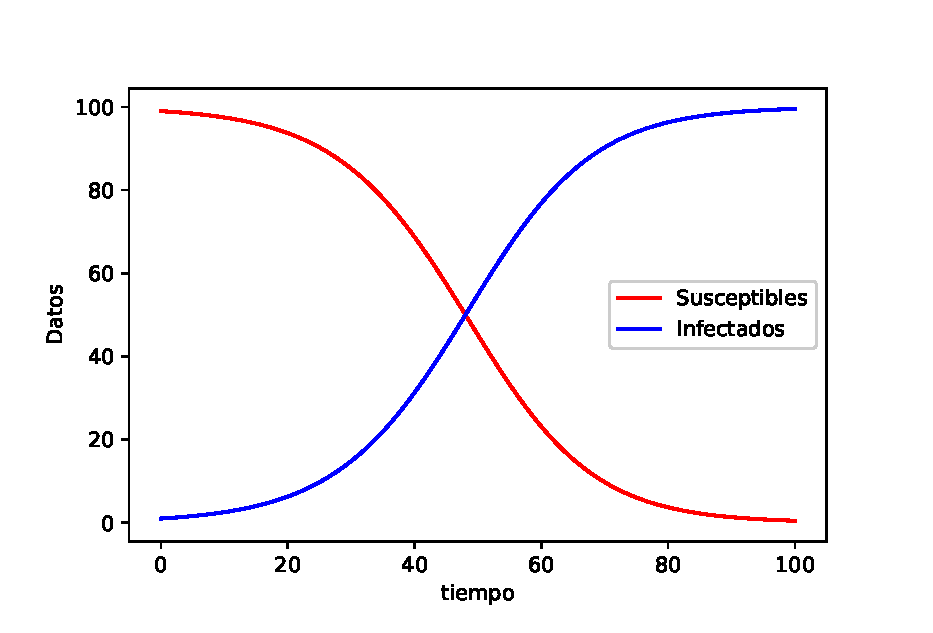
\includegraphics[scale=1]{graficaSI}
\end{center}
\end{figure}


\subsection{Modelo SIS}
Es similar al SI, pero tras infectarse los individuos vuelven a ser susceptibles.
Por ejemplo, los resfriados pueden modelarse usando SIS.

El modelo es el siguiente:

\begin{equation}
\label{eqn: modelo_SIS}
\begin{aligned}
S_{n+1} = S_n \left(1-\frac{\alpha\Delta t}{N} I_n \right) + \gamma \Delta t I_n \\
I_{n+1} = I_n \left( 1-\gamma \Delta t + \frac{\alpha\Delta t}{N} S_n \right)
\end{aligned}
\end{equation}

con condiciones iniciales positivas $S_0>0$, $I_0>0$ cumpliendo $S_0+I_0=N$. Por lo tanto, el tamaño de la población es constante.

En estas ecuaciones, $\alpha$ de nuevo representa la tasa de contacto, esto es, el número medio de individuos con los que un infectado tiene suficiente contacto para contagiarlo en un intervalo de tiempo y $\gamma$ es la probabilidad de que un infectado pase a recuperado/retirado/aislado/fallecido en un intervalo de tiempo, donde se cumple $\alpha >0$ y $\gamma >0$.

Además las soluciones siempre son positivas si, y solo si:

$$\gamma \Delta t \leq 1 $$ y $$\alpha\Delta t< \left( 1+\sqrt{\gamma \Delta t} \right)^2$$

Esto se puede consultar en el Lema 2 del Apéndice de \cite{allenDiscretetimeSISIR1994}.

\textcolor{red}{No he comprobado las cuentas de esas condiciones}

La tasa reproductiva de este modelo es $\mathcal{R}=\alpha /\gamma$ \textcolor{red}{No entiendo como saca esa tasa reproductiva, he repetido las cuentas y las de antes estaban mal. Si no es por definición como dijimos el otro día no se dónde sale}

 

\subsection{Modelo SIR}
Comienza como el SI, pero tras infectarse los individuos pasan a un estado Recuperado, en el cual no pueden infectarse ni infectar a otros.
Por ejemplo, la varicela. 

El modelo es el siguiente:

\begin{equation}
\label{eqn: SIR_modelo}
\begin{aligned}
S_{n+1} = S_n \left(1-\frac{\alpha\Delta t}{N} I_n \right) \\
I_{n+1} = I_n \left( 1-\gamma \Delta t + \frac{\alpha\Delta t}{N} S_n \right) \\
R_{n+1} = R_n + \gamma \Delta t I_n
\end{aligned}
\end{equation}

con condiciones iniciales $S_0>0$, $I_0>0$, $R_0\geq 0$, satisfaciendo $S_0+I_0+R_0=N$.

En estas ecuaciones, de nuevo tenemos que $\alpha$ es la tasa de contacto, esto es, el número medio de individuos con los que un infectado tiene suficiente contacto para contagiarlo en un intervalo de tiempo y $\gamma$ es la probabilidad de que un infectado pase a recuperado/retirado/aislado/fallecido en un intervalo de tiempo, con $\alpha >0$ y $\gamma >0$.

Se supone que la población permanece constante, $S_n+I_n+R_n=N$.

Además, tenemos que las soluciones a este sistema discreto son positivas para cualquier valor de las condiciones iniciales si, y solo si:

$$\max{\big\{\gamma\Delta t, \alpha\Delta t\big\} } \leq 1$$

o equivalentemente:

$$\min{\bigg\{ \frac{1}{\gamma}, \frac{1}{\alpha} \bigg\} } \geq \Delta t$$

Por tanto, el intervalo de tiempo debe ser menor que el tiempo medio requerido para un contacto exitoso y menor que el período medio infeccioso.
% Con contacto exitoso asumo que se refiere al tiempo necesario para infectar a un individuo. Sí es esto confirmado por la profe

El comportamiento global del sistema es fácil de ver. Sea $\mathcal{R}=S_0 \alpha/(N\gamma )$ la tasa reproductiva. \textcolor{red}{¿Por qué $\mathcal{R}$ es justo eso?}. El valor de $\mathcal{R}$ determina el comportamiento global del modelo. \textcolor{red}{(a esto después lo llamo tasa de transmisión media en el artículo \cite{demongeotSIEpidemicModel})}. 

Notemos que $S_n$ es estrictamente decreciente y $R_n$ es estrictamente creciente. Estudiémoslas:

Sea $S_\infty=\lim_{n\rightarrow\infty} S_n\geq 0$, cuyo límite existe pues es una sucesión estr4ictamente decreciente y acotada inferiormente por $0$, que depende de las condiciones iniciales. Si $S_0\leq \frac{\gamma N}{\alpha}$, o, equivalentemente, $\mathcal{R}\leq 1$ entonces $I_1\leq I_0$ y, como $S_n$ es estrictamente decreciente, tenemos que $I_{n+1}\leq I_n$, es decir, no hay epidemia. En otro caso, tenemos $S_0> \frac{\gamma N}{\alpha}$, entonces $I_1>I_0$. Debe ocurrir que $S_\infty <\frac{N\gamma}{\alpha}$, pues si no fuera así, tendríamos que $I_n$ crece hacia un equilibrio, $I_\infty$, lo que implica que $R_n$ se aproxima a infinito cuando $n\rightarrow\infty$, lo cuál no es posible. Así, el número de infectados finalmente comienza a decrecer y se aproxima a $0$. Además, sabemos por el Lema 1 de \cite{allenDiscretetimeSISIR1994} que $S_\infty>0$.

El modelo continuo se comporta de la misma forma que el modelo discreto, este sería:

\begin{equation}
\label{eqn: modelo_SIR_continuo}
\begin{cases}
\frac{dS}{dt} = -\frac{\alpha}{N}SI \\
\frac{dI}{dt} = I\left(\frac{\alpha}{N}S-\gamma \right) \\
\frac{dR}{dt} = R+\gamma I
\end{cases}
\end{equation}

donde $S(0)+I(0)+R(0)=N$. La tasa reproductiva en este caso es $\mathcal{R}=S(0)\alpha /(N\gamma )$, y si $\mathcal{R}\leq 1$  no hay epidemia, pero en cambio, si es mayor, hay epidemia.

He programado el modelo discreto y el resultado de la gráfica ha sido:

\begin{figure}
\begin{center}
\caption{Gráfica del modelo SIR, en una población total de $100$ individuos, con valores iniciales $S_0=99, I_0 = 1, R_0 = 0, \alpha = 0.1, \gamma = 0.01 T_0 = 0, T = 300$}
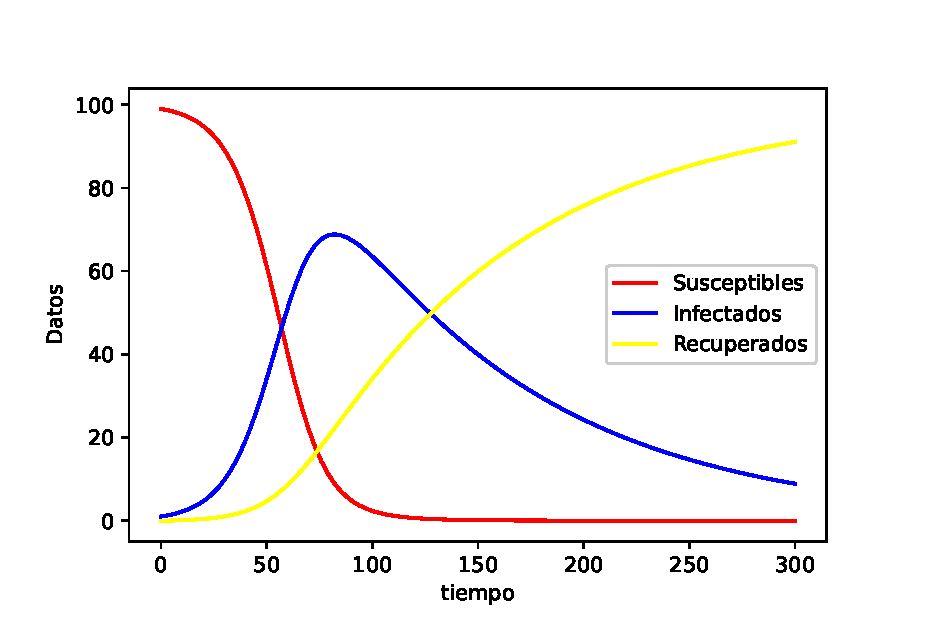
\includegraphics[scale=1]{graficaSIR}
\end{center}
\end{figure}





\section{Cosas del articulo de rsos que no sé que nombre ponerles}

\subsection{Introducción}

Estimar la tasa de transmisión media es uno de los aspectos más cruciales en epidemiología. Esta tasa condiciona la fase de la epidemia e incluso si va a extinguirse. Es combinación de tres factores:

\begin{enumerate}
\item Coeficiente de virulencia: Relacionado con el agente infeccioso.
\item Coeficiente de susceptibilidad: Relacionado con el anfitrión.
\item Número de contactos por unidad de tiempo entre individuos.
\end{enumerate}

Los dos primeros factores se tienen en cuenta a la vez en la probabilidad de transmisión.

Todos los factores pueden cambiar con el tiempo, el primero debido a mutaciones del virus y los dos últimos por medidas de contención. Por tanto, observar el decrecimiento de la transmisión media en una enfermedad es una buena forma de comprobar la efectividad de las medidas de contención.

Consideramos un modelo SI con el objetivo de compararlo con los datos obtenidos en la pandemia de la COVID-19 hasta el momento y así tratar de predecir su comportamiento en el futuro.

El modelo SI continuo es el siguiente:

\begin{equation}
\label{eqn: SI_cont}
\begin{aligned}
S'(t) = -\tau (t)S(t)I(t) \\
I'(t) = \tau (t)S(t)I(t) -vI(t)
\end{aligned}
\end{equation}

donde $S(t)$ es el número de individuos susceptibles , $I(t)$ el número de individuos infectados en el tiempo $t$ y $\tau (t)$ la tasa de transmisión, que combina el número de contactos por unidad de tiempo y la probabilidad de transmisión. Además, notemos que $v$ es constante, donde $1/v$ es la duración media del período de infección, y $vI(t)$ el flujo de individuos recuperados o fallecidos \textcolor{red}{¿Por que ese es el flujo de recuperados o muertos?}. Consideramos condiciones iniciales:

$$S(t_0)=S_0>0, \: I(t_0)=I_0>0$$

Ahora, consideramos que al final del período infeccioso nos han informado de una fracción del total de casos, en este caso $f\in (0,1]$. Sea $C_R(t)$ el número total (acumulado) de casos reportados. Entonces:

\begin{equation}
\label{eqn: acumulada}
C_R(t) = {C_R}_0 + vfC_I(t) \; \forall t \geq t_0
\end{equation}

\textcolor{red}{¿Por qué $vfC_I(t)$ va multiplicado por $v$?}

donde

$$C_I(t) = \int_{t_0}^t I(w) dw $$

Asumimos conocidos $S_0 > 0$, $1/v>0$, $f\in (0,1]$. Por tanto, queremos averiguar $I_0$, $\tau (t)$

\subsection{Aproximando $I_0$ y $\tau (t_0)$}
Ahora, procedemos a intentar aproximar $I_0$ y $\tau (t_0)$:

Al comienzo de la pandemia podemos asumir que $S(t)$ y $\tau (t)$ son constantes e iguales a $S_0$ y $\tau_0 = \tau (t_0)$ respectivamente. Así, sustituyendo estos valores en la ecuación (\ref{eqn: SI_cont}) obtenemos:

$$I'(t) = (\tau_0 S_0 -v) I(t)$$

Resolviendo la ecuación diferencial llegamos a:

$$I(t) = I_0\exp{((\tau_0 S_0-v)(t-t_0))}$$

Sustituyendo en (\ref{eqn: acumulada}):

$$C_R(t) = {C_R}_0 + vfI_0\frac{\mathrm{e}^{(\tau_0 S_0 -v)(t-t_0)} -1}{\tau_0 S_0-v}$$

Así, hemos obtenido un primer modelo para los casos acumulados al principio de la pandemia.

Reescribimos la ecuación como:

\begin{equation}
\label{eqn: acumulada_modelo}
C_R(t) = \chi_1 \mathrm{e}^{\chi_2 t} -\chi_3
\end{equation}

Estimamos $\chi_3$ usando los datos de la epidemia obtenidos, y el mejor ajuste para los datos es $\chi_3=0$

Ahora, usando (\ref{eqn: acumulada}) y (\ref{eqn: acumulada_modelo}) tenemos:

\begin{equation}
I_0=\frac{\chi_1\chi_2\mathrm{e}^{\chi_2 t_0}}{vf}
\end{equation}

Y, como de reescribir sabemos que $\chi_2 = \tau_0 S_0-v$ entonces

\begin{equation}
\tau_0 = \frac{\chi_2+v}{S_0}
\end{equation}

Si suponemos que $\tau (t) = \tau_0$ tenemos que el modelo queda:

\begin{equation}
\begin{aligned}
S'(t) = -\tau_0S(t)I(t) \\
I'(t) = \tau_0S(t)I(t) -vI(t)
\end{aligned}
\end{equation}

Usando la ecuación de $S(t)$ y resolviéndola obtenemos:

$$S(t) = S_0\exp{\left( -\tau_0 \int_{t_0}^t I(w) dw \right)} = S_0\exp{(-\tau_0 C_I(t))}$$

Ahora, sustituyendo esta expresión en la ecuación de $I(t)$ del modelo y usando $C_I'(t)=I(t)$:

$$I'(t) = S_0\exp{\left( -\tau_0 C_I(t)\right) }\tau_0 C_I'(t)-vI(t)$$

Finalmente, integrando entre $t_0$ y $t$ tenemos que:

$$I(t)=C_I'(t)=I_0+S_0(1-\exp{(-\tau_0 C_I(t)}))-vC_I(t)$$

Observamos entonces que el número total de infectados es monótono creciente (¡pero no el número de infectados!). 

\begin{theorem}
Sea $t>t_0$ fijo. El número de infectados acumulados es estrictamente creciente respecto a las siguiente cantidades:
\begin{itemize}
\item $I_0>0$ Número inicial de infectados
\item $S_0>0$ Número inicial de individuos susceptibles.
\item $\tau>0$ Tasa de transmisión
\item $1/v$ Tiempo medio de la infección.
\end{itemize}
\end{theorem}

\subsection{Fórmula teórica para $\tau (t)$}

Usando la ecuación del modelo inicial (\ref{eqn: SI_cont}) obtenemos:
% La ecuacion de la S$

$$S(t) = S_0 \exp{\left( - \int_{t_0}^t \tau(w) I(w) dw \right) } $$ 

Ahora, sustituyendo en la ecuación (\ref{eqn: SI_cont}):
% La ecuacion de la I

$$I'(t) = S_0 \exp{\left( - \int_{t_0}^t \tau(w) I(w) dw \right) } \tau (t) I(t) -vI(t) $$

Integramos en ambos lados entre $t_0$ y $t$, luego:

$$ C_I'(t) = I_0 + S_0 \left( 1-\exp{\left(- \int_{t_0}^t \tau (w) I(w)dw \right)}\right) -vC_I(t)$$

Equivalentemente, por (\ref{eqn: acumulada}):

$$C_R'(t) = vf\left( I_0 + S_0 \left( 1-\exp{\left(- \frac{1}{vf}\int_{t_0}^t \tau (w ) I(w)dw \right)}\right)\right) +v{C_R}_0 -vC_R(t)$$

\textcolor{red}{Esta cuenta no termina de salirme, pero tiene más o menos sentido}

Así, obtenemos el Teorema 3.1 de \cite{demongeotSIEpidemicModel}, que nos da la relación directa buscada.










% Part II
%\input{chapters/chapter5}

% ----------------------- %
% BIBLIOGRAFÍA
% ----------------------- %

% Estilo de cita.
\bibliographystyle{unsrtnat}

%[citestyle=numeric]

% Añadimos la bibliografía al índice
\phantomsection
\addcontentsline{toc}{chapter}{Bibliografía}

\bibliography{bib/library}

\end{document}